\documentclass[british]{report}
\usepackage{amsmath}
\usepackage{verbatim}
\usepackage{enumitem}
\usepackage{blindtext}
\usepackage{graphicx}
\usepackage{titling}
\usepackage[usenames, dvipsnames, table]{xcolor}
\usepackage{tikz}
\usepackage{float}
\usepackage{titlesec}
\usepackage{lipsum}
\usepackage{lmodern} % https://tex.stackexchange.com/a/57265

% \usepackage[colorlinks]{hyperref}
\usepackage[hidelinks]{hyperref}
\usepackage{glossaries}
\usepackage[automake]{glossaries-extra}
\usepackage{cleveref}

%Package to draw simple directory trees | https://tex.stackexchange.com/a/253595
\usepackage{dirtree}

\usepackage{babel}
\usepackage{csquotes}

\usepackage{todonotes}

\usepackage[titletoc]{appendix}

\usepackage{soul}

\usepackage{needspace}

\usepackage[datesep=/,style=ddmmyyyy]{datetime2}

\usepackage{minted}
\usemintedstyle[ts]{vs}

\usepackage{caption} % https://tex.stackexchange.com/a/112660

\usepackage{mdframed} % https://www.slideshare.net/linjaaho/how-to-make-boxed-text-with-latex slide 8

\usepackage{pdfpages} % https://stackoverflow.com/a/2739710/7193940

\usepackage{listings} % From the projectdocument


\usepackage[utf8]{inputenc}

\usepackage{bigfoot} % https://tex.stackexchange.com/a/87493

\usepackage{wrapfig} % https://tex.stackexchange.com/a/55179

\usepackage{fancyvrb} % https://tex.stackexchange.com/a/451397

% \makeatletter
% \def\@xobeysp{ } % https://web.archive.org/web/20100428131559/newsgroups.derkeiler.com/Archive/Comp/comp.text.tex/2009-04/msg00306.html
% \makeatother

\definecolor{plum}{rgb}{0.56, 0.27, 0.52} % https://latexcolor.com/
\definecolor{raspberry}{rgb}{0.89, 0.04, 0.36}
\definecolor{pear}{rgb}{0.82, 0.89, 0.19}
\newcommand{\todoil}[1]{\todo[inline]{#1}} % Add inline todo command
\newcommand{\todoilq}[1]{\todo[inline, color=raspberry!100]{#1}} % Add purple inline todo command
\newcommand{\todoq}[1]{\todo[color=raspberry!100]{#1}} % Add purple inline todo command
\newcommand{\todoref}{\todo[color=pear!100]{Add ref}}

% Todonotes doc 1.8.13: Highlight text to fix
\makeatletter
	\if@todonotes@disabled
		\newcommand{\todohl}[2]{#1}
	\else
		\newcommand{\todohl}[2]{\sethlcolor{yellow}\texthl{#1}\todo{#2}}
		\newcommand{\todohlq}[2]{\sethlcolor{yellow}\texthl{#1}\todo[color=raspberry!100]{#2}}
	\fi
\makeatother

\usepackage[
backend=biber,
%style=alphabetic,
sorting=none, %anyvt
datamodel=lastedit,
lasteditdate=short,
maxbibnames=99, % https://tex.stackexchange.com/a/1557
]{biblatex}

\addbibresource{bibliography.bib}

% https://tex.stackexchange.com/a/412669
\NewBibliographyString{lastchanged}
\DefineBibliographyStrings{english}{
  lastchanged = {last changed},
}

% \DeclareFieldFormat{lasteditdate}{\mkbibparens{\bibstring{lastchanged}\space#1}}

% \renewbibmacro*{url+urldate}{%
%   \usebibmacro{url}%
%   \iffieldundef{lastedityear}
%     {}
%     {\setunit*{\addspace}%
%      \printlasteditdate}%
%   \iffieldundef{urlyear}
%     {}
%     {\setunit*{\addspace}%
%      \usebibmacro{urldate}}}

\titleformat{\chapter}[display]
{\normalfont\huge\bfseries}{\chaptertitlename\ \thechapter}{20pt}{\Huge}

% this alters "before" spacing (the second length argument) to 0
\titlespacing*{\chapter}{0pt}{0pt}{10pt}

% https://tex.stackexchange.com/a/7549
\newcommand{\latex}{\LaTeX\xspace}
\newcommand{\tex}{\TeX\xspace}

\makeglossaries

\newlength\longest % https://tex.stackexchange.com/a/57265

\pretitle{%
    \definecolor{fontys}{RGB}{102,51,102}
    
    % upper triangle
    \begin{tikzpicture}[remember picture, overlay, shift={(current page.north west)}]
        
        \node (p0) at (0.0,                     0.0) {};
        \node (p1) at (\paperwidth + 20.0cm,    0.0) {};
        \node (p2) at (0.0,                     -4.0) {};
      
        \fill[fontys]
        (p0.center)--(p1.center)--(p2.center);
        
    \end{tikzpicture}
    
    
    % content
    \begin{figure}[ht]
        \centering
        \vspace{-75mm}
        \protect
\includegraphics[width=100mm]{figures/00-FONTYS-CARD_CARD-WIT-RGB.jpg}
        %\vspace{-30mm}
    \end{figure}
   
    % lower triangle
    \begin{tikzpicture}[remember picture, overlay, shift={(current page.south west)}]
        
        \node (p0) at (-60.0,       0.0) {};
        \node (p1) at (\paperwidth, 0.0) {};
        \node (p2) at (\paperwidth, 10.0) {};
      
        \fill[fontys]
        (p0.center)--(p1.center)--(p2.center);
        
    \end{tikzpicture}

    \begin{center}
}
\title{
    \huge \textbf{Swagshop writeup} \\
    \vspace{5mm}
    \large Hack the Box \\
    \url{https://www.hackthebox.eu/home/machines/profile/188}\\
    \vspace{5mm}
    \textit{Report for Fontys Hogeschool ICT}
    \normalsize
}
    
\author{Jort Geurts | i360843 | 3007235}

\posttitle{\end{center}}

%%%%%%%%%%%%%%%%%%%%%%%%%%%%%%%%%%%%%%%%%%%%%%%%%%%%%
%					ABREVIATIONS					%
%%%%%%%%%%%%%%%%%%%%%%%%%%%%%%%%%%%%%%%%%%%%%%%%%%%%%

%\newabbreviation{abbrv}{ABBRV}{Abbrevation That Matters}

\newabbreviation{api}{API}{Application Programming Interface}
\newabbreviation{sqli}{SQLi}{SQL injection}
\newabbreviation{cms}{CMS}{Content Management System}
\newabbreviation{rce}{RCE}{Remote Code Execution}

% \gls{fms}

%%%%%%%%%%%%%%%%%%%%%%%%%%%%%%%%%%%%%%%%%%%%%%%%%%%%%
%					 GLOSSARIES						%
%%%%%%%%%%%%%%%%%%%%%%%%%%%%%%%%%%%%%%%%%%%%%%%%%%%%%

\newglossaryentry{git}{name=git, description={``A version control system for tracking changes in computer files and coordinating work on those files among multiple people." \cite{git}}}

\newglossaryentry{cve}{name=CVE, plural=CVEs, description={The Common Vulnerabilities and Exposures system is a way to responsibly document and provide reference for vulnerabilities found in public systems.}}

\begin{document}

\nocite{*}

\maketitle

\newpage

% \clearpage

\thispagestyle{empty}
\null\vfill

\settowidth\longest{\Large\itshape The internet gave us access to everything;}
\begin{center}
\parbox{\longest}{%
  \raggedright{\Large\itshape%
   The internet gave us access to everything; \\ 
  but it also gave everything access to us.\par\bigskip
  }   
  \raggedleft\MakeUppercase{James Veitch}\par%
}
\end{center}

% https://www.ted.com/talks/james_veitch_the_agony_of_trying_to_unsubscribe/transcript
% https://tex.stackexchange.com/a/57265

\vfill\vfill

\clearpage
\newpage
\addtocontents{toc}{\protect\setcounter{tocdepth}{2}}
\tableofcontents

\newpage

\printglossaries

\newpage

\chapter{Basic information}
\label{chap:info}

The specs of this box are:

\begin{table}[H]
    \begin{tabular}{ll}
    Name:       & SwagShop          \\
    OS:         & Linux             \\
    Difficulty: & Easy              \\
    Points:     & 20                \\
    Release:    & 11 May 2019       \\
    Retirement: & 28 September 2019 \\
    IP:         & 10.10.10.140      \\
    Retired:    & Yes               \\
    URL:        & \url{https://www.hackthebox.eu/home/machines/profile/188}
    \end{tabular}
\end{table}

\noindent Time until user pwn: $\pm 10$ hours\\
Time until root pwn: $\pm 40$ hours (including scripting the user shell)

\vspace{5mm}

\noindent User flag: \verb|a448877277e82f05e5ddf9f90aefbac8|\\
Root flag: \verb|c2b087d66e14a652a3b86a130ac56721|

\begin{comment}
    <referenceContainer name="sidebar.additional">
   <block class="Magento\Backend\Block\Template" name="test">
      <action method="fetchView">
         <argument name="fileName" xsi:type="string">/var/www/html/Theme/view/frontend/../../../../../../pub/media/custom_options/quote/r/e/7a38695d69c295652a6c5cb4a8843dd3.phtml</argument>
      </action>
   </block>
</referenceContainer> 

<referenceContainer name="sidebar.additional">
   <block class="Magento\Backend\Block\Template" name="test">
      <action method="fetchView">
         <argument name="fileName" xsi:type="string">/var/www/html/app/code/Magento/Theme/view/frontend/../../../../../../pub/media/custom_options/quote/r/e/7a38695d69c295652a6c5cb4a8843dd3.phtml</argument>
      </action>
   </block>
</referenceContainer>
\end{comment}

\chapter{Basic recon}
\label{chap:basic_recon}

As per usual when you get a box, the first step is to find as much information about it as you can. A quick \verb|nmap| reveals that port 80 and 22 are open. Http and ssh. Going to the ip in a browser shows a Magento webshop, with three items pre-configured. After some basic \gls{sqli} attempts, I decide that it's probably gonna be a bit more complex than that.

Then the hunt starts. The specs of the box say that \glspl{cve} are a big part of this box, so I start looking around for relevant \glspl{cve}. Not knowing what version of Magento is used, it was kind of a spray method. I noticed that the copyright was on 2014, so it's very likely that it's an older version.

There are two Magento versions, v1 and v2. I was still unsure what version was used, so I was just trying some exploits I could find. The exploits on \url{https://www.exploit-db.com/} turned out to be really useful, and it had a script (\#37977) to get a login on the admin dashboard. This script worked, and the admin page was on the default location (\verb|10.10.10.140/index.php/admin|).

\begin{figure}[H]
	\centering
	\captionsetup{justification=centering}
	\noindent 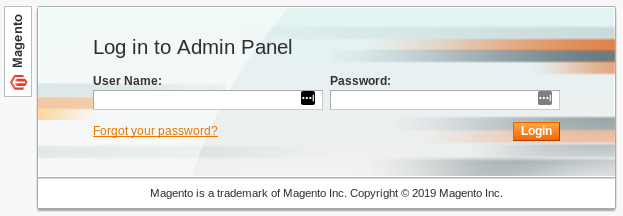
\includegraphics[width=\textwidth]{figures/magento-login.png}
	\caption{\emph{The login page of Magento}}
	\label{fig:magentologin}
\end{figure}

The admin page turned out to contain the version number of Magento, \verb|v|. This meant I could pin my exploit search to a specific version. After searching through the \gls{cms} for quite some time for interesting ways in, I was unsure where the exploit would be.

\vspace{5mm}

There was a lot written about exploiting a downloader included in Magento, but, after some reading on the HTB forums, I found out that this downloader was disabled because it was an unintentional way in.

Then I looked at exploit \#37811, hoping this would be it. I found\\ \verb|http://10.10.10.140/app/etc/local.xml|, giving me the install date, which could be used in the script. However, after running, with some slight modifications I got it to a point where it would crash with the error seen in \cref{fig:37811.py}. Searching for this error actually brings up the HTB forums for this challenge, stating that I should stop looking. It was apparently not the way forward.

\begin{figure}
	\centering
	\captionsetup{justification=centering}
	\noindent 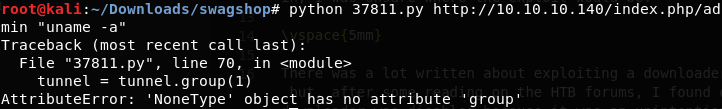
\includegraphics[width=\textwidth]{figures/python-37811-tunnel-error.png}
	\caption{\emph{The python script crashing}}
	\label{fig:37811.py}
\end{figure}

\chapter{Exploit 1}
\label{chap:exploit1}

After a lot of DuckDuckGo-ing, I found the blogpost which ended up giving a solution. The blog can be found here: \url{https://blog.scrt.ch/2019/01/24/magento-rce-local-file-read-with-low-privilege-admin-rights/}. Recently, a \gls{rce} was found which abused the way custom XML can be used in Magento. In this case, the path to uploading the malicious PHP script and executing it is divided into two steps.

\section{Uploading the script}

The python script mentioned in \cref{chap:basic_recon} was used to gain admin access to the \gls{cms}. I then followed the following steps:

\vspace{5mm}

Firstly, I created a new product.\footnote{\verb|Catalog > Manage Products > Add Product|} A 'Simple Product' is enough. I entered some dummy information to fill in all the fields, because the product itself doesn't matter. But, there is a way to add an upload form to a product. This is our way in.

\begin{figure}[H]
	\centering
	\captionsetup{justification=centering}
	\noindent 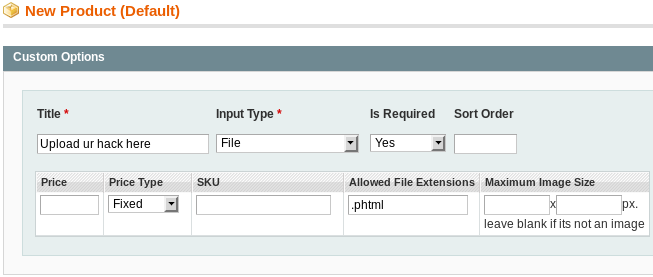
\includegraphics[width=\textwidth]{figures/new-product-upload.png}
	\caption{\emph{The way to add an upload form to a product page.}}
	\label{fig:37811.py}
\end{figure}

So, now that we have a way to upload our reverse shell PHP file to the server, we need to trick the server into executing it. The aforementioned blogpost does this via an XML trick.

Here I deviate from the blog post a little. In the used version of Magento I couldn't find the mentioned `design tab' on the product page, so I started to look for other ways that I could give custom \verb|Layout Update XML|. I found that creating new page\footnote{\verb|CMS > Pages|} also provided the option to give custom XML\footnote{\verb|CMS > Pages > New Page > Design > Page Layout|}.

Then I had to figure out where the uploaded \verb|.phtml| file actually was placed on the filesystem. I made a guess that it'd be the default installation, so \verb|/var/www/html|. This was correct, and I obtained my reverse shell using \\\verb|nc -v -n -l -p 10365|.

\vspace{5mm}

However, then disaster struck. I had obtained the reverse shell, but after I submitted the user flag, I had left it alone. I hadn't documented the exact XML I used, and the server was reset by someone else. I had lost my reverse shell. I tried to do every step again, but I couldn't get it to work again. To this day I have no clue what was different in that specific instance of the server. I suspect another user had already changed some settings, which allowed this hack to work.

\begin{figure}[H]
	\centering
	\captionsetup{justification=centering}
	\noindent 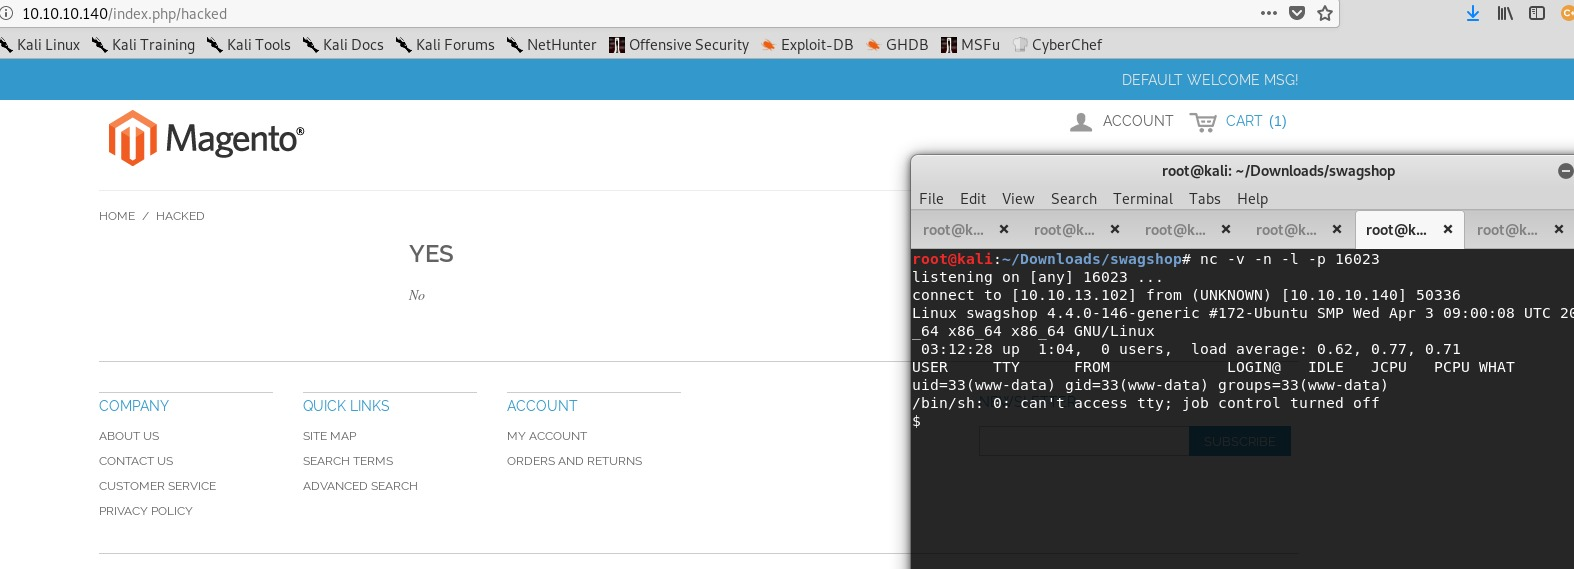
\includegraphics[width=\textwidth]{figures/exploit-1.jpeg}
	\caption{\emph{Screenshot of the initial shell I obtained.}}
	\label{fig:exploit1}
\end{figure}

\chapter{Exploit 2}
\label{chap:exploit2}

So with the first exploit no longer working, I was determined to find another way. I started to message around on the HTB forums, to see if someone had found the same way; and could tell me what I was doing wrong. I got a response outlining another way to get a reverse shell into the server, so I started to work on that.

\vspace{3mm}

The blogpost from the first exploit also mentioned another file-read exploit with the email templates. However, there is another issue with the newsletter templates. Apparently, they are also capable of executing \verb|.phtml| files.

The initial exploit to gain admin access was the same, as I already expected. However, he (ab)uses the image-upload functionality given when you create a category. The instructions I got were quite bare, so I had to do some figuring out on how to exactly exploit this.

\vspace{3mm}

I started with a lot of DuckDuckGo-ing, figuring out how to include a malicious PHP script into an image. I found that there are two main\footnote{More information and two other ways: \\\url{https://hackers2devnull.blogspot.com/2013/05/how-to-shell-server-via-image-upload.html}} ways:

\begin{itemize}
    \item Firstly, you can add a small PHP script to the EXIF data of the image, basically giving it a description with a PHP script. The issue with this method is that this doesn't give a full reverse shell.
    \item Secondly, you can rename the PHP script, and try to trick the website into thinking you uploaded an image; whilst in reality it's a script. This can give a proper full shell, since you can upload any PHP script this way.
\end{itemize}

\begin{wrapfigure}{r}{3.5cm}
	\centering
	\captionsetup{justification=centering, font=small}
	\noindent 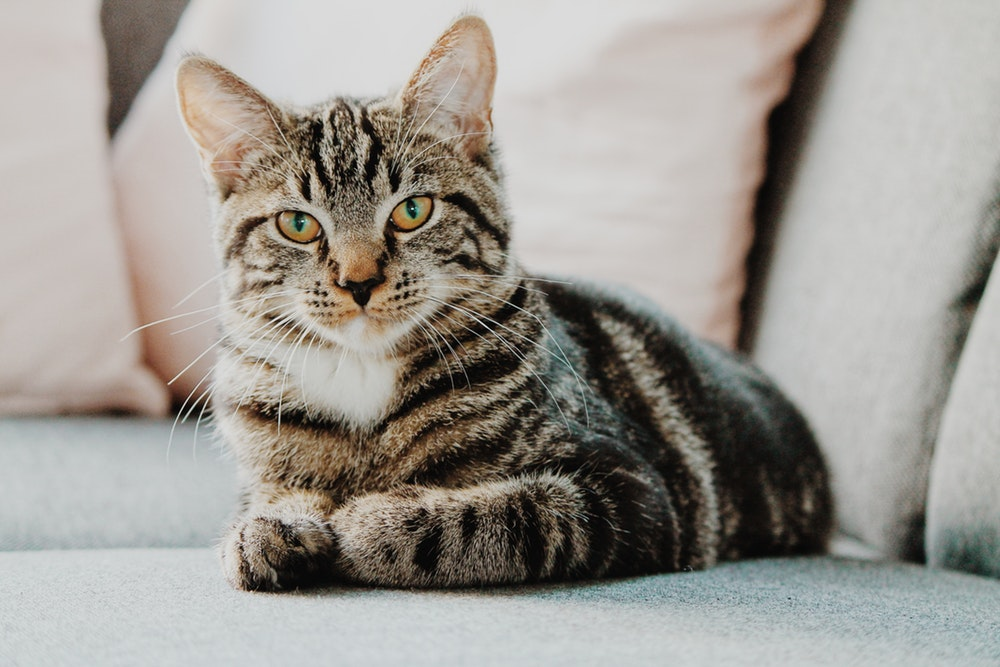
\includegraphics[width=\linewidth]{figures/cat.jpeg}
	\caption{\scriptsize{\emph{The cute cat picture I used for testing.}}}
	\label{fig:cat}
\end{wrapfigure}

So I decided to start with the second option, since it seemed like the easier one. I copied my reverse shell script a few times, using some of the suggestions from the blogpost found in the footnote. I uploaded them, but I wasn't sure if I'd get feedback from the site if it succeeded. Then I started to doubt whether the traversal from the second step would even work, so I used the cute cat picture seen in \cref{fig:cat} for a test.

Doing this, I found out that this trick indeed actually works. The raw image is displayed, indicating to me that this might be susceptible to executing code. After this I started to try more strange extensions, finding out that \verb|.php.jpg| worked. I knew this, because it showed up after I uploaded the file.

On to the second stage, the execution of the script. I got hinted towards another issue with the newsletter templates. Including the following code would allow me to traverse to the saved PHP script, and it should be executed via the 'Preview Template': 

\begin{Verbatim}[breaklines=true, breakanywhere=true]
    {{block type='core/template' template='../../../../../../media/catalog/category/reverse_shell.php.jpg}}
\end{Verbatim}

Another setting that needed to be changed was to allow symlinks. This setting can be found under \verb|System > Developer > Template Settings|. I suspect this allows the path traversing that is used in the path to the `image'.

The template could then be executed via the `Preview Template' option. This way, the server would show an iframe with the email content; including the `image'. The page would show an infinite loading screen, which is normal behavior for the reverse shell script.

\chapter{The script}
\label{chap:script}

So, this box has a tendency to be resetted a lot. On average, this machine gets reset over a hundred times a day. Apart from this, \verb|script kiddies| keep launching automated attacks, crippeling the server. This makes it really difficult to keep your shell on the machine. So, as part of the requirement \verb|Automating offensive security tasks.|, I decided to write a custom Python script, to automatically re-gain my shell.

\vspace{5mm}

This was easier said than done. I knew the steps that I had to take, but it this total undertaking took me about a week to complete. This was partly due to my inexperience in Python, partly due to weird documentation of the scraping plugin, \verb|BeautifulSoup| and partly due to some bad API behavior of Magento.

\vspace{5mm}

I am aware that the code quality isn't the highest. Some things could be more fail-proof, tho I've tried to write the code flexible enough that it should work on other machines with the same vulnerable Magento version. Also, the script can be ran multiple times on the same machine without any negative effect.

This is because all the custom things I upload are using UUID's as filenames, meaning they're practically unique. This way there are no collisions in namings on the server, with the newly created category, uploaded exploit and created newsletter template.

\vspace{5mm}

\noindent In broad lines, the script does the following:

\begin{itemize}
    \item Uses the \verb|37977.py| script to gain admin credentials to the server.
    \item Logs in to the server, and using the \verb|Session| functionality from the \verb|requests| package; I'm able to keep the session going between requests.
    \item Disables the url-keys. This means the requests don't have to be appended with a random key. This has the advantage that I don't need to scrape myself through the site, but I can just directly make the requests I need.
    \item Enabling symlinks, this is a requirement for the traversal in a later stage of the exploit.
    \item Next, I create the category with an unique UUID, and upload the PHP exploit.
    \item Then, I have to create the newsletter template, with the right code inside referring to the uploaded PHP exploit from the previous step.
    \item Finally, the newsletter template needs to be 'previewed' to run the exploit.
\end{itemize}

As with every piece of code, there were a thousand different challenges involved in this. Traversing though the scraped html code was a huge challenge. Since this is so error-prone, I wanted to do this with as much built-in flexibility as possible.

Another thing that was new to me, is that all the settings are sent to the server in a \verb|multipart form data| form. I had never heard of this, and had to research how this method of transferring data works, and how to do it in Python.

The server refused to apply the settings if the request contained a \verb|filename| attribute, so I had to strip that out. Figuring this out, and figuring out how to do its was already a few hours down the drain. In the end, the solution ended up being a structure like this:

\begin{listing}
    \begin{minted}[linenos, breaklines, breakautoindent=true]{python}
        multipart_form_data = {
            'form_key': (None, system_config_form_key),
            'groups[security][fields][use_form_key][value]': (None, 0)
        }
    
        response = session.post(url + '/admin/system_config/save/section/admin/key/' + urlKey + '/', files=multipart_form_data)
    
    \end{minted}
    \caption{\emph{Python code used to make a valid request to change a setting (disabling the url-keys).}}
\end{listing}



The \verb|'thing': (None, value)| ended up being the solution. The None apparently means that it isn't a file, meaning that it won't send the \verb|filename| attribute.

\chapter{The flags}
\label{chap:flags}

So, now that I have a reverse shell; how do I get the user and root flag? Luckily this first is rather easy. The reverse shell already gives me access to an user, \verb|www-data|. All that was left for this flag was to traverse to the \verb|/user/harim| folder, which would hold the \verb|user.txt| flag.

\vspace{5mm}

One flag down, one flag to go.

\section{Root}

The search for root started with the \verb|sudo -l| command. This listed that the current user (\verb|www-data|) had rights to use sudo without a password for \verb|/usr/bin/vi| and \verb|/var/www/html/*|. Vi being the famous text editor, and the html folder in which the Magento installation resides.

\begin{figure}[H]
	\centering
	\captionsetup{justification=centering}
	\noindent 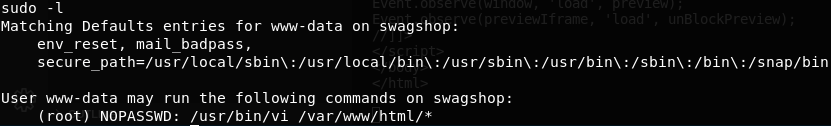
\includegraphics[width=\textwidth]{figures/sudo-output.png}
	\caption{\emph{The output of sudo -l.}}
	\label{fig:sudo}
\end{figure}

I figured this was no coincidence, and this would be the pivoting point to root. After some duckduckgo-ing around, I found an article on Medium\footnote{\url{https://link.medium.com/0dwd0VgL7Z}} about using Vim for privilege escalation. The user in the screenshots was \verb|haris|, which I suspect is actually this box.

The final example is about vim, and the output of \verb|sudo -l| actually looked really similar to mine. But this is where I went wrong, because the command \verb|sudo vi| didn't work. So I thought this was wrong, and started looking for other ways in.

\vspace{5mm}

In the end, I only had a few hours left before the box would be retired to find the root flag. I started to ask around on the Hack the Box forums, hoping to find some help to find the root flag. I got again nudged towards the sudoers file and Vim, which confused me. So, after a lot of playing around I found what I did wrong.

\begin{center}
    \verb|sudo vi| doesn't work. \verb|sudo /usr/bin/vi| does.
\end{center}

\begin{wrapfigure}{r}{4.5cm} % 4.5cm
	\centering
	\captionsetup{justification=centering}
	\noindent 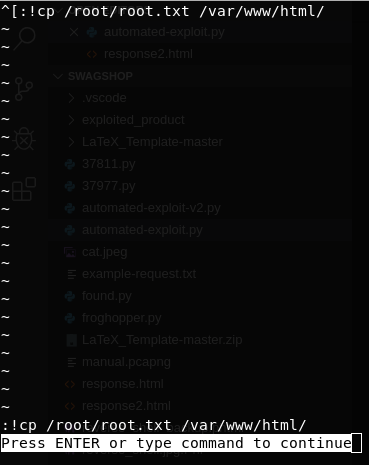
\includegraphics[width=\linewidth]{figures/root-copy-2.png}
	\caption{\emph{How I copied the file from within Vim.}}
	\label{fig:vimcopy}
\end{wrapfigure}

\vspace{2mm}

So, simple solution right? Just open the \verb|/root/root.txt| file with \verb|sudo /usr/bin/vi| and you have your flag. No. This actually was not allowed for some reason. So, what I ended up doing was copying the \verb|/root/root.txt| file to the \verb|/var/www/html| folder, and opening it there. This ended up giving me the root flag.

\begin{figure}[H]
	\centering
	\captionsetup{justification=centering}
	\noindent 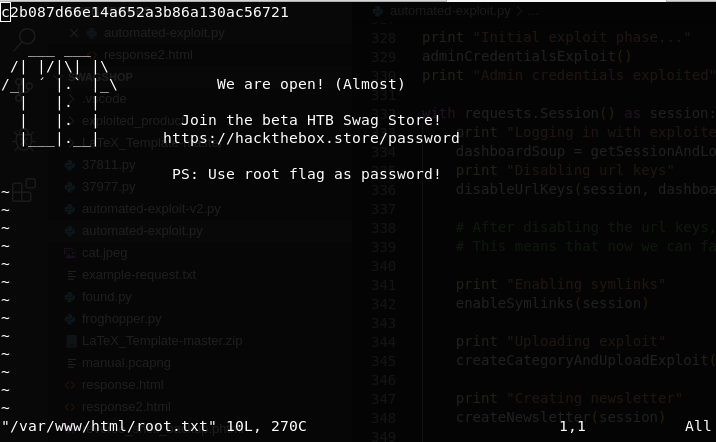
\includegraphics[width=\textwidth]{figures/root.png}
	\caption{\emph{The content of the root.txt file.}}
	\label{fig:root}
\end{figure}

% More content

% \newpage
% \printbibliography

% \listoftodos

\end{document}